\documentclass[]{BasiliskReportMemo}
\usepackage{cite}
\usepackage{AVS}
\usepackage{float} %use [H] to keep tables where you put them
\usepackage{array} %easy control of text in tables
\usepackage{graphicx}
\bibliographystyle{plain}



\newcommand{\submiterInstitute}{Autonomous Vehicle Simulation (AVS) Laboratory,\\ University of Colorado}

\newcommand{\ModuleName}{MRP\_Feedback}
\newcommand{\subject}{MRP Feedback ADCS Control Module}
\newcommand{\status}{Initial Documentation Draft}
\newcommand{\preparer}{H. Schaub}
\newcommand{\summary}{This module provides a general MRP feedback control law, applying to using $N$ reaction wheels with general orientation.     }


\begin{document}


\makeCover


%
%	enter the revision documentation here
%	to add more lines, copy the table entry and the \hline, and paste after the current entry.
%
\pagestyle{empty}
{\renewcommand{\arraystretch}{2}
\noindent
\begin{longtable}{|p{0.5in}|p{4.5in}|p{1.14in}|}
\hline
{\bfseries Rev}: & {\bfseries Change Description} & {\bfseries By} \\
\hline
Draft & Initial Draft document & H. Schaub \\
\hline

\end{longtable}
}

\newpage
\setcounter{page}{1}
\pagestyle{fancy}

\tableofcontents
~\\ \hrule ~\\

\begin{figure}[htb]
	\centerline{
	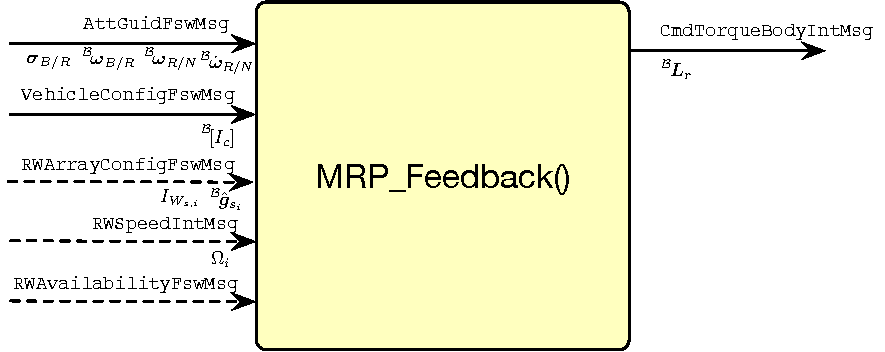
\includegraphics[]{Figures/moduleIO}
	}
	\caption{{\tt MRP\_Feedback()} Module I/O Illustration}
	\label{fig:moduleIO}
\end{figure}
\section{Module Description}
The {\tt MRP\_Feedback} module creates the MRP attitude feedback control torque $\bm L_{r}$ developed in chapter 8 of Reference~\citenum{schaub}.  The input and output messages are illustrated in Figure~\ref{fig:moduleIO}.  The output message is a body-frame control torque vector that is outlined in section~\ref{sec:alg}.  The required attitude guidance message contains both attitude tracking error states as well as reference frame states.  This message is read in with every update cycle. The vehicle configuration message is only read in on reset and contains the spacecraft inertia tensor about the vehicle's center of mass location.  

The MRP feedback control can compensate for Reaction Wheel (RW) gyroscopic effects as well.  This is an optional input message where the RW configuration array message contains the RW spin axis $\hat{\bm g}_{s,i}$ information and the RW polar inertia about the spin axis $I_{W_{s,i}}$.  This is only read in on reset.  The RW speed message contains the RW speed $\Omega_{i}$ and is read in every time step.  The optional RW availability message can be used to include or not include RWs in the MRP feedback.  This allows the module to selectively turn off some RWs.  The default is that all RWs are operational and are included.  



\section{Initialization}
Simply call the module reset function prior to using this control module.  This will reset the prior function call time variable, and reset the attitude error integral measure.  The control update period $\Delta t$ is evaluated automatically.  

\section{Algorithm}\label{sec:alg}
		 This module employs the MRP feedback algorithm of Example 8.14 of Reference \citenum{schaub}.  This  nonlinear attitude tracking control includes an integral measure of the attitude error.  Further, we seek to avoid quadratic $\bm\omega$ terms to reduce the likelihood of control saturation during a detumbling phase.  Let the new nonlinear feedback control be expressed as
		\begin{equation}
			\label{eq:GusRW}
			[G_{s}]\bm u_{s} = -\bm L_{r} 
		\end{equation}
		where
		\begin{multline}
			\label{eq:Lr}
			\bm L_{r} =  -K \bm\sigma - [P] \delta\bm\omega - [P][K_{I}] \bm z  - [I_{\text{RW}}](-\dot{\bm\omega}_{r} + [\tilde{\bm\omega}]\bm\omega_{r}) - \bm L
			\\
			+ ([\tilde{\bm \omega}_{r}] + [\widetilde{K_{I}\bm z}])
			\left([I_{\text{RW}}]\bm\omega + [G_{s}]\bm h_{s} \right)
		\end{multline}
		and 
		\begin{equation}
			h_{s_{i}} = I_{W_{s_{i}}} (\hat{\bm g}_{s_{i}}^{T} \bm\omega_{B/N} + \Omega_{i})
		\end{equation}
		with $I_{W_{s}}$ being the RW spin axis inertia.

		The integral attitude error measure $\bm z$ is defined through
		\begin{equation*}
			\bm z = K \int_{t_{0}}^{t} \bm\sigma \text{d}t + [I_{\text{RW}}](\delta\bm\omega - \delta\bm\omega_{0})
		\end{equation*}
		In the BSK module the vector $\delta\bm\omega_{0}$ is hard-coded to a zero vector.  This function will work for any initial tracking error, and this assumption doesn't impact performance.
		
		The integral measure $\bm z$ must be computed to determine $[P][K_{I}] \bm z$, and the expression $[\widetilde{K_{I}\bm z}]$ is added to $[\widetilde{\bm\omega_{r}}]$ term.  

		To analyze the stability of this control, the following Lyapunov candidate function is used:
		\begin{equation*}
			V(\delta\bm\omega, \bm\sigma, \bm z) = \frac{1}{2} \delta\bm\omega^{T} [I_{\text{RW}}] \delta\bm\omega
			+ 2 K \ln ( 1 + \bm\sigma^{T} \bm\sigma) + \frac{1}{2} \bm z ^{T} [K_{I}]\bm z
		\end{equation*}
		provides a convenient positive definite attitude error function.  The attitude feedback gain $K$ is positive, while the integral feedback gain $[K_{I}]$ is a symmetric positive definite matrix.  
		The resulting Lyapunov rate expression, solved in Eq.~(8.101), is given by
		\begin{equation*}
			\dot V =  (\delta\bm\omega + [K_{I}]\bm z)^{T} \left ( [I_{\text{RW}}] \frac{{}^{\mathcal{B \!}}\text{d}}{\text{d}t} (\delta\bm\omega) + K \bm \sigma \right )
		\end{equation*}
		Substituting the equations of motion of a spacecraft with $N$ reaction wheels (see Eq.~(8.160) in Reference~\citenum{schaub}), results in
		\begin{equation*}
			\dot V =  (\delta\bm\omega + [K_{I}]\bm z )^{T} \left (
			 - [\tilde{\bm\omega}] ([I_{\text{RW}}] \bm\omega +[G_{s}]\bm h_{s}) - [G_{s}] \bm u_{s} + \bm L
			 - [I_{\text{RW}}] ( \dot{\bm \omega}_{r} - [\tilde{\bm\omega}]\bm\omega_{r}) + K \bm\sigma
			\right)
		\end{equation*}
		Substituting the control expression in Eq.~\eqref{eq:GusRW} and making use of $\bm \alpha = \bm\omega_{r} - [K_{I}]\bm z$ leads  to 
		\begin{align*}
			\begin{split}
			\dot V &=  (\delta\bm\omega + [K_{I}]\bm z )^{T} \Big (
			- ([\tilde{\bm\omega}] - [\tilde{\bm\omega}_{r}] + [\widetilde{K_{I}\bm z}]) ([I_{\text{RW}}] \bm\omega + [G_{s}]\bm h_{s})
			+( K \bm\sigma - K \bm\sigma) 
			\\
			& \quad - [P]\delta\bm\omega - [P][K_{I}]\bm z + [I_{\text{RW}}](\dot{\bm\omega}_{r} - [\tilde{\bm\omega}]\bm\omega_{r}) - [I_{\text{RW}}](\dot{\bm\omega}_{r} - [\tilde{\bm\omega}]\bm\omega_{r})
			+ ( \bm L - \bm L)
			\Big)
			\end{split}
			\\
			&=  (\delta\bm\omega + [K_{I}]\bm z )^{T} \Big (
			 - ([\widetilde{\delta\bm\omega}] + [\widetilde{K_{I}\bm z}] )  ([I_{\text{RW}}] \bm\omega + [G_{s}]\bm h_{s})
			 - [P] (\delta\bm\omega + [K_{I}]\bm z)
			\Big )
		\end{align*}
		Because $(\delta\bm\omega + [K_{I}]\bm z )^{T}  ([\widetilde{\delta\bm\omega}] + [\widetilde{K_{I}\bm z}] ) = 0$, the Lyapunov rate reduces the negative semi-definite expression
		\begin{equation*}
			\dot V = -  (\delta\bm\omega + [K_{I}]\bm z )^{T} [P]  (\delta\bm\omega + [K_{I}]\bm z )
		\end{equation*}
		This proves the new control is globally stabilizing.  Asymptotic stability is shown following the same steps as for the  nonlinear integral feedback control in Eq. (8.104) in Reference~\citenum{schaub}.  
		
		One of the goals set forth at the beginning of the example was avoiding quadratic $\bm\omega$ feedback terms to reduce the odds of control saturation during periods with large $\bm\omega$ values.  However, the control in Eq.~\eqref{eq:GusRW} contains a product of $\bm z$ and $\bm\omega$.  Let us study this term in more detail.  The $\bm\omega$ expression with this product terms is found to be
		\begin{equation*}
			[\widetilde{K_{I}\bm z}] ([I_{\text{RW}}]\bm \omega)
			 \quad \Rightarrow \quad 
			-  (
			[\widetilde{I_{\text{RW}} \bm \omega}] 
			 ) ([K_{I}] [I_{\text{RW}}] \bm \omega + \cdots )
		\end{equation*}
		If the integral feedback gain is a scalar $K_{I}$, rather than a symmetric positive definite matrix $[K_{I}]$, the quadratic $\bm\omega$ term vanishes.  If the full $3\times 3$ gain matrix is employed, then quadratic rate feedback terms are retained.  

\section{Unit Test}
The unit test for this module \verb|test_MRP_feedback| tests a set of gains $K,K_i,P$ on a rigid body with no external torques, and with a fixed input reference attitude message. The torque requested by the controller is evaluated against python computed torques at 0s, 0.5s, 1s, 1.5s and 2s to within a tolerance of $10^{-8}$. After 1s the simulation is stopped and the Reset() function is called to check that integral feedback related variables are properly reset.  The following permutations are run:
\begin{itemize}
	\item The test is run for a case with error integration feedback ($k_i=0.01$) and one case where $k_i$ is set to a negative value, resulting in a case with no integrator. 
	\item The RW array number is configured either to 4 or 0
	\item The integral limit term is set to either 0 or 20
	\item The RW availability message is tested in 3 manners.  Either the availability  message is not written where all wheels should default to being available.  If the availability message is written, then the RWs are either zero to available or not available.
	\item The control parameter $\delta\omega_{0}$ is set to either a zero or non-zero vector
\end{itemize}
All permutations of these test cases are expected to pass.





\section{User Guide}
This module requires the following variables:
\begin{itemize}
\item $\mathbf{\sigma}_{BN}$ as \verb|guidCmdData.sigma_BR|
\item $^B\mathbf{\omega}_{BR}$  as \verb|guidCmdData.omega_BR_B|
\item $^B\mathbf{\omega}_{RN}$ as \verb|guidCmdData.omega_RN_B|
\item $^B\dot{\mathbf{\omega}}_{RN}$ as \verb|guidCmdData.domega_RN_B|
\item $[I]$, the inertia matrix of the body as \verb|vehicleConfigOut.ISCPntB_B|
\item $\Omega_i$, speed of each reaction wheel in \verb|rwSpeedMessage.wheelSpeeds|
\item Gains $k,P$ in \verb|moduleConfig|. 
\item The integral gain $K_i$ in \verb|moduleConfig|. Setting this variable to a negative number disables the error integration for the controller, leaving just PI terms. Zero is not supported as a value for $k_i$. This variable is used to compute the integralLimit, used to limit the degree of integrator windup and reduce the chance of controller saturation. The integrator is required to maintain asymptotic tracking in the presence of an external disturbing torque.
\end{itemize}



\bibliographystyle{unsrt}   % Number the references.
\bibliography{references}   % Use references.bib to resolve the labels.


\end{document}
